\documentclass[11pt]{article}

% Page layout
\usepackage[a4paper, margin=1in]{geometry}

% Math packages
\usepackage{amsmath, amssymb, amsfonts}

% Typography
\usepackage{lmodern}
\usepackage{microtype}

% Diagrams
\usepackage{tikz}
\usetikzlibrary{arrows.meta}

% Spacing
\usepackage{setspace}
\setstretch{1.1}
\setlength{\parindent}{0pt}
\setlength{\parskip}{6pt}

% Lists & tables
\usepackage{enumitem}
\setlist{noitemsep}
\usepackage{array}
\usepackage{booktabs}

% Colors & boxes
\usepackage{xcolor}
\usepackage[most]{tcolorbox}

% Links
\usepackage[hidelinks]{hyperref}

% Section styling
\usepackage{titlesec}
\titleformat{\section}{\Large\bfseries}{}{0em}{}
\titleformat{\subsection}{\large\bfseries\color{black!80}}{}{0em}{}

% Commands
\newcommand{\N}{\mathbb{N}}
\newcommand{\Z}{\mathbb{Z}}
\newcommand{\Q}{\mathbb{Q}}
\newcommand{\R}{\mathbb{R}}
\newcommand{\C}{\mathbb{C}}

% Colors
\definecolor{myblue}{HTML}{D6EAF8}
\definecolor{myred}{HTML}{FADBD8}
\definecolor{mypurple}{HTML}{E8DAEF}

% Boxes
\newtcolorbox{theorybox}{
    colback=mypurple,
    colframe=purple!70!black,
    title=\textbf{Theory},
    breakable,
    arc=6pt
}

\newtcolorbox{remarkbox}{
    colback=myblue,
    colframe=blue!60!black,
    title=\textbf{Remarks},
    breakable,
    arc=6pt
}

\newtcolorbox{problembox}{
    colback=myred,
    colframe=red!70!black,
    title=\textbf{Problems},
    breakable,
    arc=6pt
}

% Separator
\newcommand{\sepline}{
    \vspace{0.5em}
    \hrule
    \vspace{1em}
}

\begin{document}

% TITLE PAGE

\begin{titlepage}
    \centering
    
    \vspace*{3cm}
    
    {\Huge \bfseries How Numbers Work \par}
    
    \vspace{0.5cm}
    {\Large Sets, Properties and Extensions \par}
    
    \vspace{1.5cm}
    
    {\large Lostless1907 \par}
    {\large March 2026 \par}

    \vspace{1.5cm}

    \textbf{Legend}

    \vspace{0.5cm}

    \begin{tcolorbox}[colback=mypurple,colframe=purple!70!black,width=0.6\textwidth]
    \centering \textbf{Theory}
    \end{tcolorbox}

    \begin{tcolorbox}[colback=myblue,colframe=blue!60!black,width=0.6\textwidth]
    \centering \textbf{Remarks}
    \end{tcolorbox}

    \begin{tcolorbox}[colback=myred,colframe=red!70!black,width=0.6\textwidth]
    \centering \textbf{Problems}
    \end{tcolorbox}

    \vfill
    
    \sepline
    
    {\large \textit{A structured exploration of number systems for all the dedicated self-learners} \par}

\end{titlepage}

\newpage

% PREFACE

\section*{Preface}
\sepline

\subsection*{Introduction}

Numbers form a foundational layer of mathematical thought. 
This handout presents number systems as a sequence of necessary extensions, 
each introduced to resolve a limitation of the previous one.

\subsection*{Sets}

A \textbf{set} is a collection of objects, called \textit{elements}. 
If $x$ belongs to a set $A$, we write:
\[
x \in A
\]

\subsection*{A Note on Relations}

A \textbf{relation} on a set assigns a condition between elements. 
A special type, called an \textbf{equivalence relation}, satisfies:

For $a,b,c \in \N$, equality defines an equivalence relation:

\begin{itemize}
    \item $a = a$ \hfill (reflexivity)
    \item $a = b \implies b = a$ \hfill (symmetry)
    \item $a = b,\; b = c \implies a = c$ \hfill (transitivity)
\end{itemize}

Such relations group elements into \textbf{equivalence classes}, 
where elements are considered “the same” under the relation. 

\begin{remarkbox}
We will use equivalence classes of pairs $(a,b) \in \N \times \N$ 
to construct a system where subtraction is always possible.
\end{remarkbox}

\subsection*{\textsc{The Culprits}}

We will work with five primary number systems:

\begin{itemize}
    \item $\N$ — Natural Numbers
    \item $\Z$ — Integers
    \item $\Q$ — Rational Numbers
    \item $\R$ — Real Numbers
    \item $\C$ — Complex Numbers
\end{itemize}

\begin{remarkbox}
Each system arises to fix a limitation:
\[
\N \rightarrow \Z \rightarrow \Q \rightarrow \R \rightarrow \C
\]
\end{remarkbox}

% NATURALS

\section*{\textsc{Meet the Naturals}}
\sepline

\begin{theorybox}

The natural numbers are the most intuitive number system:
\[
\N = \{1,2,3,\dots\}
\]

They satisfy:

\begin{itemize}
    \item \textbf{Unboundedness:} For any $M \in \R$, there exists $n \in \N$ such that $n > M$.
    
    \item \textbf{Well-ordering:} Every non-empty subset of $\N$ has a least element.
    
    \item \textbf{Closure:} If $a,b \in \N$, then $a+b \in \N$ and $ab \in \N$.
    
    \item \textbf{Commutativity:}
    \[
    a+b = b+a, \quad ab = ba
    \]
    
    \item \textbf{Associativity:}
    \[
    a+(b+c) = (a+b)+c
    \]
    
    \item \textbf{Distributivity:}
    \[
    a(b+c) = ab + ac
    \]
\end{itemize}

\end{theorybox}

\begin{center}
\begin{tikzpicture}[scale=1]
\draw[->] (0,0)--(6,0);
\foreach \x in {1,...,5}
\draw (\x,0.1)--(\x,-0.1) node[below]{\x};
\node at (3,0.5) {$\N$};
\end{tikzpicture}
\end{center}

\begin{remarkbox}
The natural numbers support addition and multiplication, but not subtraction in general. 
This limitation motivates the construction of the integers $\Z$.
\end{remarkbox}

\begin{problembox}

\textbf{Where $\N$ Breaks}

\begin{enumerate}

\item For which natural numbers $a,b \in \N$ is $a - b$ also in $\N$?  
What happens when $b > a$?

\item Consider the equation:
\[
x + 3 = 1
\]
Does this have a solution in $\N$?

\item Try to solve:
\[
x + a = b
\]
for arbitrary $a,b \in \N$.  
When does a solution exist in $\N$?

\item Define a relation on pairs $(a,b) \in \N \times \N$:
\[
(a,b) \sim (c,d) \iff a + d = b + c
\]

\begin{itemize}
\item Show this is an equivalence relation.
\item Compute:
\[
(3,1), \quad (4,2), \quad (5,3)
\]
What do you notice?
\end{itemize}

\item Consider pairs $(a,b)$ as representing a “difference” $a - b$.  
Show that:
\[
(a,b) \sim (c,d) \implies a - b = c - d
\]

\item Define addition on pairs:
\[
(a,b) + (c,d) = (a+c, b+d)
\]

Show that this respects the relation $\sim$.

\item Find a pair $(a,b)$ such that:
\[
(a,b) + (b,a) \sim (0,0)
\]

What does this suggest?

\item Is there a pair $(a,b)$ such that:
\[
(a,b) \sim (0,0)
\]
What does this represent?

\item Show that for any $(a,b)$, there exists another pair that “cancels” it under addition.

\item Challenge:  
Construct a system of numbers using pairs $(a,b) \in \N \times \N$ 
that allows subtraction to always be possible. Define it like we defined N.

\end{enumerate}

\end{problembox}

\section*{\textsc{Meet the Integers}}
\sepline

\begin{theorybox}

The natural numbers fail to solve equations of the form:
\[
a + x = b \quad \text{when } b < a
\]

To resolve this, we extend $\N$ to a larger system:
\[
\Z = \{\dots, -2, -1, 0, 1, 2, \dots\}
\]

\textbf{What $\Z$ fixes and introduces:}

\begin{enumerate}

\item \textbf{Solvability of Equations}

For all $a,b \in \Z$, the equation
\[
a + x = b
\]
always has a solution:
\[
x = b - a
\]

\item \textbf{Bidirectional Infinity}

Unlike $\N$, which extends only to the right, $\Z$ extends infinitely in both directions:
\[
\dots < -2 < -1 < 0 < 1 < 2 < \dots
\]

\item \textbf{Order but not Well-Ordering}

$\Z$ is ordered, but not well-ordered:
there is no smallest element due to negative infinity.

\item \textbf{Successors and Predecessors}

Every integer has both:
\[
\text{successor: } n+1, \quad \text{predecessor: } n-1
\]

\item \textbf{Closure under Addition and Subtraction}

For all $a,b \in \Z$:
\[
a + b \in \Z, \quad a - b \in \Z
\]

In particular, subtraction is now always possible.

\item \textbf{Sign Structure}

For $a,c \in \N$, define $x = -a$. Then:
\[
x + c = (-a) + c =
\begin{cases}
c - a & \text{if } c \ge a \\
-(a - c) & \text{if } a > c
\end{cases}
\]

\item \textbf{Algebraic Laws Still Hold}

For all $a,b,c \in \Z$:

\textbf{Commutativity:}
\[
a+b = b+a, \quad ab = ba
\]

\textbf{Associativity:}
\[
a+(b+c) = (a+b)+c
\]

\textbf{Distributivity:}
\[
a(b+c) = ab + ac
\]

\item \textbf{Identity Elements}

There exist special elements:
\[
a + 0 = a, \quad a \cdot 1 = a
\]

\item \textbf{Additive Inverses}

For every $a \in \Z$, there exists $-a \in \Z$ such that:
\[
a + (-a) = 0
\]

\end{enumerate}

\end{theorybox}

\begin{center}
\begin{tikzpicture}[scale=1]
\draw[->] (-4,0)--(4,0);
\foreach \x in {-3,...,3}
\draw (\x,0.1)--(\x,-0.1) node[below]{\x};
\node at (0,0.7) {$\Z$};
\end{tikzpicture}
\end{center}

\begin{remarkbox}

The integers do more than fix subtraction in $\N$.

They ensure that equations of the form $a + x = b$ are always solvable, 
even when both $a$ and $b$ lie outside $\N$.

However, this extension comes with a tradeoff:  
$\Z$ is no longer well-ordered.

This reflects a general principle:

\textit{Extending a number system increases solvability, 
but may sacrifice certain structural properties.}

\end{remarkbox}

\begin{problembox}

\textbf{What $\Z$ Fixes}

\begin{enumerate}

\item Consider the equation:
\[
x + 5 = 2
\]
Explain why this has no solution in $\N$, but does in $\Z$.

\item More generally, for $a,b \in \N$, determine when:
\[
x + a = b
\]
has a solution in $\N$.  
What must be added to always solve it?

\item Show that for every $a \in \Z$, there exists $x \in \Z$ such that:
\[
a + x = 0
\]
What does this element represent?

\item Prove that subtraction can be rewritten as:
\[
a - b = a + (-b)
\]
Why is this not always possible in $\N$?

\item Show that for any $a,b \in \Z$:
\[
a - b = 0 \iff a = b
\]

\item Prove that:
\[
-(a + b) = (-a) + (-b)
\]

\item Show that:
\[
(-1)\cdot a = -a
\]
for all $a \in \Z$.

\item Prove that:
\[
(-a)(-b) = ab
\]

\item Show that if $a + b = a + c$, then $b = c$.  
(Why does this rely on additive inverses?)

\item Prove that $\Z$ is closed under subtraction.  
Why is this property new compared to $\N$?

\item Show that $\Z$ is not well-ordered.  
(Find a subset with no least element.)

\item Show that for every $n \in \Z$, both $n+1$ and $n-1$ exist in $\Z$.  
Why is this different from $\N$?

\item Prove that:
\[
|a+b| \le |a| + |b|
\]
for all $a,b \in \Z$.

\item Show that:
\[
a^2 \ge 0
\]
for all $a \in \Z$, and determine when equality holds.

\item Challenge:  
Show that there is no integer between $n$ and $n+1$ for any $n \in \Z$.  
Compare this with what happens in $\Q$.

\end{enumerate}

\end{problembox}

\begin{remarkbox}

The rationals do more than fix division in $\Z$.

They ensure that equations of the form $ax = b$ are always solvable 
for $a \neq 0$.

Unlike $\Z$, this extension does not sacrifice order, 
but introduces a new phenomenon:

between any two rational numbers, there are infinitely many others.

This reflects a general pattern:

\textit{Each extension increases solvability and density, 
while preserving as much structure as possible.}

\end{remarkbox}

\section*{\textsc{Meet the Rationals}}
\sepline

\begin{theorybox}

The integers solve subtraction, but still fail to solve equations of the form:
\[
ax = b \quad \text{when } a \nmid b
\]

To resolve this, we extend $\Z$ to:
\[
\Q = \left\{ \frac{a}{b} \;\middle|\; a,b \in \Z,\; b \neq 0 \right\}
\]

\textbf{Definition and Structure}

\begin{enumerate}

\item \textbf{Fractions as Solutions}

The expression $\frac{a}{b}$ is defined to be the solution of:
\[
bx = a
\]

Thus, division is introduced as the inverse of multiplication.

\item \textbf{Equivalence of Fractions}

Two fractions represent the same number if:
\[
\frac{a}{b} = \frac{c}{d} \iff ad = bc
\]

This ensures consistency of representation.

\item \textbf{Scaling Property}

For any nonzero $p \in \Z$:
\[
\frac{a}{b} = \frac{pa}{pb}
\]

Thus, a rational number has infinitely many representations.

\item \textbf{Sign Convention}

\[
\frac{-a}{b} = \frac{a}{-b}
\]

We usually write the negative sign in the numerator:
\[
-\frac{a}{b}
\]

If both are negative:
\[
\frac{-a}{-b} = \frac{a}{b}
\]

\item \textbf{Operations are Well-Defined}

Addition:
\[
\frac{a}{b} + \frac{c}{d} = \frac{ad + bc}{bd}
\]

Multiplication:
\[
\frac{a}{b} \cdot \frac{c}{d} = \frac{ac}{bd}
\]

These are \textbf{well-defined}, meaning:
they do not depend on the chosen representation.

\item \textbf{Why Multiplication is Meaningful}

Since $\frac{a}{b}$ represents the solution to $bx = a$, multiplying two rationals corresponds to combining two such scalings:
\[
\frac{a}{b} \cdot \frac{c}{d} = \frac{ac}{bd}
\]

This preserves the structure of solving equations of the form $ax = b$.

\item \textbf{Closure}

For all $x,y \in \Q$:
\[
x+y \in \Q, \quad xy \in \Q, \quad x \neq 0 \implies \frac{1}{x} \in \Q
\]

\item \textbf{Algebraic Laws}

All familiar laws extend from $\Z$:

\begin{itemize}
    \item Commutativity
    \item Associativity
    \item Distributivity
\end{itemize}

\item \textbf{Identity Elements}

\[
x + 0 = x, \quad x \cdot 1 = x
\]

\item \textbf{Multiplicative Inverses}

For $x \neq 0$:
\[
x \cdot \frac{1}{x} = 1
\]

\end{enumerate}

\end{theorybox}

\begin{remarkbox}

The rationals introduce a major structural shift:

\begin{itemize}

\item \textbf{Density:}  
Between any two rational numbers, there are infinitely many others.  
Unlike $\N$ and $\Z$, $\Q$ has no notion of a “next” element.

\item \textbf{Arbitrary Precision:}  
Rational numbers can approximate quantities as closely as desired:
\[
\frac{1}{3},\; \frac{33}{100},\; \frac{333}{1000}, \dots
\]

\item \textbf{Closure of Division:}  
For $a \neq 0$, the equation $ax = b$ always has a solution in $\Q$.

\item \textbf{Multiple Representations:}  
Each rational number has infinitely many forms:
\[
\frac{1}{2} = \frac{2}{4} = \frac{50}{100}
\]

\end{itemize}

\end{remarkbox}

\textit{We also, for rigour and the topic's interestingness seemingly, include:}

\begin{theorybox}

\textbf{Density of $\Q$}

Let $x,y \in \Q$ with $x < y$.  
Then there exists $r \in \Q$ such that:
\[
x < r < y
\]

\textbf{Proof:}

Take:
\[
r = \frac{x+y}{2}
\]

Since $\Q$ is closed under addition and division by $2$:
\[
r \in \Q
\]

Also:
\[
x < \frac{x+y}{2} < y
\]

Thus, there exists at least one rational between any two rationals.

Repeating this process shows there are infinitely many.

\end{theorybox}

\begin{center}
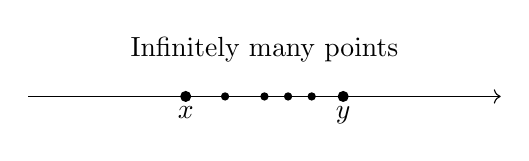
\begin{tikzpicture}[scale=1]
\draw[->] (0,0)--(6,0);

\fill (2,0) circle (2pt) node[below]{$x$};
\fill (4,0) circle (2pt) node[below]{$y$};

\foreach \p in {2.5,3,3.3,3.6}
\fill (\p,0) circle (1.5pt);

\node at (3,0.6) {Infinitely many points};
\end{tikzpicture}
\end{center}

\begin{problembox}

\textbf{Why $\Q$ Exists}

\begin{enumerate}

\item Consider the equation:
\[
2x = 1
\]
Does this have a solution in $\Z$?  
What kind of number would solve it?

\item More generally, for $a,b \in \Z$, when does:
\[
ax = b
\]
have a solution in $\Z$?

\item Show that if $a \nmid b$, then no integer solution exists to $ax=b$.  
What does this suggest we need to add?

\item Consider two pairs $(a,b)$ and $(c,d)$ with $b,d \neq 0$.  
Define:
\[
(a,b) \sim (c,d) \iff ad = bc
\]

\begin{itemize}
\item Show this is an equivalence relation.
\item What does each equivalence class represent?
\end{itemize}

\item Show that:
\[
\frac{1}{2} = \frac{2}{4} = \frac{3}{6}
\]
Explain why infinitely many representations exist.

\item Show that:
\[
\frac{a}{b} = \frac{pa}{pb}
\]
for any nonzero $p \in \Z$.

\item Show that:
\[
\frac{-a}{b} = \frac{a}{-b}
\]
and explain why we usually keep the negative sign in the numerator.

\item Define addition on pairs:
\[
(a,b) + (c,d) = (ad+bc, bd)
\]

Show that this respects the relation $\sim$.

\item Define multiplication on pairs:
\[
(a,b)(c,d) = (ac, bd)
\]

Show that this is well-defined.

\item Find a rational number strictly between:
\[
\frac{1}{2} \quad \text{and} \quad \frac{2}{3}
\]

Can you find infinitely many?

\item Show that between any two rational numbers $x < y$, there exists another rational number.

\item Challenge:  
Find a rational number between $x$ and $y$ that is \textbf{not} their midpoint.

\item Show that no matter how close two rational numbers are, there is always another rational between them.

\item Show that $\Q$ has no “next” element:
there is no smallest rational greater than a given rational.

\item Challenge (important):  
Is there a rational number whose square is $2$?  
What does your answer suggest?

\end{enumerate}

\end{problembox}

\begin{remarkbox}

Despite their richness, the rationals are still incomplete.

There exist numbers that cannot be expressed as $\frac{a}{b}$:
\[
x^2 = 2 \quad \text{has no solution in } \Q
\]

Thus, even though $\Q$ is dense, it still contains “gaps”.

This motivates the next extension: the real numbers $\R$.

\end{remarkbox}

\section*{\textsc{Meet the Reals}}
\sepline

\textbf{A Fundamental Limitation of $\Q$}

\textbf{Claim:} $\sqrt{p}$ is irrational for any prime $p$.

\textbf{Proof:}

Assume $\sqrt{p} = \frac{a}{b}$ in lowest terms, with $a,b \in \Z$.

Then:
\[
p = \frac{a^2}{b^2} \implies a^2 = p b^2
\]

So $p \mid a^2 \implies p \mid a$.

Let $a = pk$. Then:
\[
a^2 = p^2 k^2 = p b^2 \implies p k^2 = b^2
\]

Thus $p \mid b^2 \implies p \mid b$.

So $p$ divides both $a$ and $b$, contradicting that $\frac{a}{b}$ was in lowest terms.

Hence $\sqrt{p} \notin \Q$.

\subsection*{Irrational Numbers}

A number is called \textbf{irrational} if it cannot be written as:
\[
\frac{a}{b}, \quad a,b \in \Z
\]

Thus:
\[
\R = \Q \cup \{\text{irrational numbers}\}
\]

\subsection*{The Number Line}

The real numbers correspond to points on a continuous line.

Unlike $\Q$, which leaves gaps, $\R$ fills every point.

Thus, $\R$ represents the \textbf{maximal extension of number as magnitude}.

\subsection*{Dedekind's Construction}

Early Mathematician and very interesting and influential person Richard Dedekind defined Real Nos. like this.

A real number can be defined as a partition of $\Q$ into two sets:

\[
\Q = L \cup U
\]

such that:

\begin{itemize}
    \item $L$ contains all numbers less than the real number
    \item $U$ contains all numbers greater than it
    \item $L$ has no greatest element
\end{itemize}

Example: $\sqrt{2}$ corresponds to:
\[
L = \{x \in \Q : x^2 < 2\}, \quad U = \{x \in \Q : x^2 > 2\}
\]

\begin{theorybox}

The real numbers extend $\Q$ by eliminating all gaps.

\[
\R = (-\infty, \infty)
\]

\textbf{What $\R$ fixes and introduces:}

\begin{enumerate}

\item \textbf{Completeness}

Every bounded set has a least upper bound.

\item \textbf{No Gaps}

All limits of converging sequences in $\Q$ exist in $\R$.

\item \textbf{Closure}

For $x,y \in \R$:
\[
x+y, \; xy \in \R
\]

\item \textbf{Order}

$\R$ is totally ordered.

\item \textbf{Algebraic Laws}

All standard laws hold.

\item \textbf{Continuity}

$\R$ forms a continuous number line.

\end{enumerate}

\end{theorybox}

\begin{center}
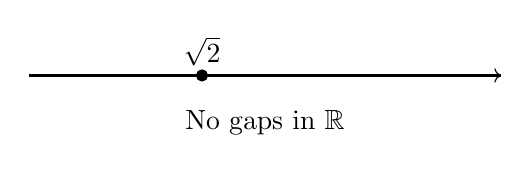
\begin{tikzpicture}[scale=1]
\draw[->] (0,0)--(6,0);

\draw[thick] (0,0)--(6,0);

\filldraw (2.2,0) circle (2pt) node[above]{$\sqrt{2}$};

\node at (3,-0.6) {No gaps in $\R$};
\end{tikzpicture}
\end{center}

\begin{remarkbox}

The real numbers represent a fundamental leap.

While $\Q$ is dense, it is still incomplete.  
$\R$ removes this limitation entirely.

\textbf{Uncountability:}

The set $\Q$ is countable, but $\R$ is not.

This means there are strictly more real numbers than rational numbers.

Intuitively:
no matter how many rationals we list, there will always be real numbers missing.

Thus, most real numbers are irrational.

\textbf{Significance:}

$\R$ is the foundation of:
\begin{itemize}
    \item calculus
    \item analysis
    \item geometry
\end{itemize}

\end{remarkbox}

\textit{For a small taste of higher mathematics we include:}

\begin{remarkbox}

\textbf{Idea of Uncountability (Diagonal Argument)}

Assume all real numbers in $(0,1)$ can be listed.

Construct a new number by changing the $n$-th digit of the $n$-th number.

This new number differs from every number in the list.

Thus, no list can capture all real numbers.

\end{remarkbox}

\begin{problembox}

\textbf{Why $\R$ Exists}

\begin{enumerate}

\item Show that there is no rational number whose square is $2$.  
What does this imply about $\Q$?

\item Consider the set:
\[
S = \{x \in \Q : x^2 < 2\}
\]

\begin{itemize}
\item Show that $S$ is bounded above in $\Q$.
\item Does $S$ have a least upper bound in $\Q$?
\end{itemize}

What does this suggest?

\item Find a sequence of rational numbers that gets closer and closer to $\sqrt{2}$.  
Does it ever reach it in $\Q$?

\item Show that between any two real numbers, there exists a rational number.  
(Why does this not contradict density of $\Q$?)

\item Show that between any two real numbers, there exists an irrational number.

\item Show that $\R$ has no “gaps”:  
intuitively explain why every point on the number line corresponds to a real number.

\item Consider a bounded set $A \subset \R$.  
What might it mean for $A$ to have a “least upper bound”?

Give examples.

\item Find a set of rational numbers that is bounded but has no maximum.

What happens to this set in $\R$?

\item Show that:
\[
|x| = 0 \iff x = 0
\]
for all $x \in \R$.

\item Show that:
\[
|x+y| \le |x| + |y|
\]

(Why is this inequality important?)

\item Show that if $x^2 < 0$, then $x \notin \R$.  
What does this suggest about the next extension?

\item Challenge:  
Find two real numbers $x < y$ such that there are infinitely many rational numbers and infinitely many irrational numbers between them.

\item Challenge (deep):  
Construct a number by taking an infinite decimal:
\[
0.101001000100001\dots
\]
Is this rational or irrational?

\end{enumerate}

\end{problembox}




\section*{\textsc{Meet the Complexes}}
\sepline

The complex numbers are the most complete system we study.

Unlike previous extensions, $\C$ is not merely about fixing an operation —  
it ensures that \textbf{all polynomial equations have solutions}.

Thus, $\C$ is the natural endpoint of algebraic extension and is central to higher mathematics.

\begin{theorybox}

We define a number $i$ such that:
\[
i^2 = -1
\]

A complex number is of the form:
\[
z = x + iy, \quad x,y \in \R
\]

Thus:
\[
\C = \{x + iy \mid x,y \in \R\}
\]

\textbf{Algebra}

For $z_1 = a+bi,\; z_2 = c+di$:

\[
z_1 + z_2 = (a+c) + (b+d)i
\]

\[
z_1 z_2 = (ac - bd) + (ad+bc)i
\]

\textbf{Properties}

\begin{itemize}
\item Commutativity
\item Associativity
\item Distributivity
\end{itemize}

\[
\R \subset \C
\]

\[
z + 0 = z, \quad z \cdot 1 = z
\]

\end{theorybox}

\subsection*{Real and Imaginary Parts}

\[
\text{Re}(z) = x, \quad \text{Im}(z) = y
\]

\subsection*{Conjugates}

\[
\bar{z} = x - iy
\]

\[
z\bar{z} = x^2 + y^2
\]

\begin{theorybox}

\textbf{Deeper into $\C$}

\begin{itemize}
\item $\C$ is algebraically closed
\item No order relation exists compatible with multiplication
\item Sequences behave component-wise as in $\R$
\end{itemize}

\textbf{Complex Plane}

Each $z = x+iy$ corresponds to a point $(x,y)$.

\textbf{Modulus}

\[
|z| = \sqrt{x^2 + y^2}
\]

\textbf{Argument}

Angle $\theta$ such that:
\[
z = |z|(\cos\theta + i\sin\theta)
\]

\end{theorybox}

\begin{center}
\begin{tikzpicture}[scale=1]

\draw[->] (-3,0)--(3,0) node[right]{Re};
\draw[->] (0,-3)--(0,3) node[above]{Im};

\filldraw[blue] (2,1) circle (2pt) node[right]{$z$};

\draw[dashed] (2,1)--(2,0);
\draw[dashed] (2,1)--(0,1);

\draw[->,thick] (0,0)--(2,1);

\node at (1,1.2) {$|z|$};

\end{tikzpicture}
\end{center}

\begin{problembox}

\textbf{Thinking in $\C$}

\begin{enumerate}

\item Let $z = a + bi$. Show that:
\[
z = 0 \iff a = 0 \text{ and } b = 0
\]

\item Show that complex addition corresponds to vector addition in the plane.

\item Show that multiplication by $i$ rotates any complex number by $90^\circ$.

\item Describe geometrically the set:
\[
\{z \in \C : |z| = r\}
\]

\item Describe:
\[
\{z \in \C : |z - a| = r\}
\]

What does this represent?

\item Show that:
\[
|z+w| \le |z| + |w|
\]

Compare this with the real case.

\item Show that:
\[
|z-w| = |w-z|
\]

What geometric meaning does this have?

\item Find all $z \in \C$ such that:
\[
|z| = |z - 1|
\]

(What geometric object is this?)

\item Show that if $|z| = 1$, then:
\[
\bar{z} = \frac{1}{z}
\]

\item Show that:
\[
z + \frac{1}{z} \in \R \quad \text{if } |z| = 1
\]

\item Solve:
\[
z^2 = -1
\]

Then solve:
\[
z^2 = i
\]

What pattern do you observe?

\item Show that every complex number has exactly two square roots (except $0$).

\item Show that:
\[
|z|^2 = z\bar{z}
\]

Why is this important?

\item Show that multiplication in $\C$ corresponds to:
\begin{itemize}
\item scaling (changing magnitude)
\item rotation (changing angle)
\end{itemize}

\item Challenge:  
Find all $z \in \C$ such that:
\[
z^3 = 1
\]

Describe their geometric arrangement.

\item Challenge (very important):  
Show that there is no ordering on $\C$ compatible with addition and multiplication.

Why does this mean $\C$ is fundamentally different from $\R$?

\item Challenge (insight):  
Consider repeated multiplication by $i$:
\[
1, i, -1, -i, 1, \dots
\]

Explain this cycle geometrically.

\end{enumerate}

\end{problembox}

\begin{remarkbox}

Complex numbers unify algebra and geometry:

\begin{itemize}
\item Addition behaves like vector addition
\item Multiplication corresponds to rotation and scaling
\item $i$ represents a $90^\circ$ rotation
\end{itemize}

\end{remarkbox}

\begin{remarkbox}

\textbf{Comparison of Number Systems}

\begin{tabular}{lccccc}
\toprule
Property & $\N$ & $\Z$ & $\Q$ & $\R$ & $\C$ \\
\midrule
Addition & \checkmark & \checkmark & \checkmark & \checkmark & \checkmark \\
Subtraction & $\times$ & \checkmark & \checkmark & \checkmark & \checkmark \\
Division & $\times$ & $\times$ & \checkmark & \checkmark & \checkmark \\
Density & $\times$ & $\times$ & \checkmark & \checkmark & \checkmark \\
Completeness & $\times$ & $\times$ & $\times$ & \checkmark & \checkmark \\
Algebraic Closure & $\times$ & $\times$ & $\times$ & $\times$ & \checkmark \\
\bottomrule
\end{tabular}

\end{remarkbox}

\begin{problembox}

\textbf{Thinking in $\C$ (Core)}

\begin{enumerate}

\item Solve $x^2 + 1 = 0$ in $\C$
\item Show $|z|^2 = z\bar{z}$
\item Show multiplication by $i$ rotates by $90^\circ$
\item Solve $z^2 = i$
\item Find all $z$ such that $|z| = 1$

\end{enumerate}

\end{problembox}

\begin{problembox}

\textbf{Parting Shots}

\begin{enumerate}

\item Show $\sqrt{2}$ is irrational
\item Find a rational between $\frac{1}{3}$ and $\frac{1}{2}$
\item Show $\Q$ is dense
\item Show $\Q$ is countable
\item Show $\R$ is uncountable

\item Construct an irrational number
\item Show $\R$ has no gaps
\item Solve $x^2 = -1$
\item Solve $z^2 = -4$
\item Solve $z^3 = 1$

\item Show $|z|^2 = z\bar{z}$
\item Show $|zw| = |z||w|$
\item Describe $|z| = 1$
\item Describe $|z - 1| = 2$

\item Show $\C$ has no order relation

\item Find all solutions of $z^2 = i$
\item Show every quadratic has solutions in $\C$

\item Challenge: classify $0.1010010001\dots$
\item Challenge: construct infinitely many rationals between two numbers

\item Challenge (diagram):

\begin{center}
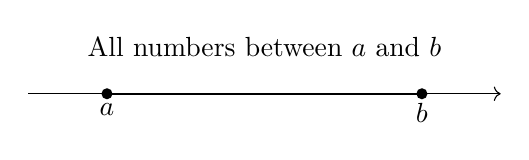
\begin{tikzpicture}
\draw[->] (-1,0)--(5,0);

\fill (0,0) circle (2pt) node[below]{$a$};
\fill (4,0) circle (2pt) node[below]{$b$};

\draw[thick] (0,0)--(4,0);

\node at (2,0.6) {All numbers between $a$ and $b$};

\end{tikzpicture}
\end{center}

\end{enumerate}

\end{problembox}

\sepline

\section{Homework aside from Problems}

Write a 300-400 word 3 para essay:

- How it was pedagogically and mathematically to do this.
- What can be improved
- What all in Math/CS Theory y'all would like next

\sepline

\section*{A Note from the Author}
\sepline

This handout was created independently.

For questions, solutions or improvements:

\begin{itemize}
\item Email: \texttt{cowboyhehe1@gmail.com}
\item GitHub: \texttt{www.github.com/Lostless1907}
\end{itemize}

Please send:
\begin{itemize}
\item Clear images or typed work
\item Suggestions or corrections
\end{itemize}

Read the \texttt{README.md} before using the source.

This is a living document, feedback and change is welcome.

\sepline

\textit{"And you, my father, there on the sad height, \\
Curse, bless, me now with your fierce tears, I pray. \\
Do not go gentle into that good night. \\
Rage, rage against the dying of the light." \\
\textbf{— With Love, VPS}}

\end{document}
